\section{Результаты}
Сравним результаты рендеринга одного и того же кадра с использованием алгоритма $SSAA$ и без его использования, а также кадры сгенерированные на $CPU$ и на $GPU$

\textbf{Примеры работы программы:}
\begin{center}

\begin{figure}[h!]
    \ContinuedFloat*
    \centering
    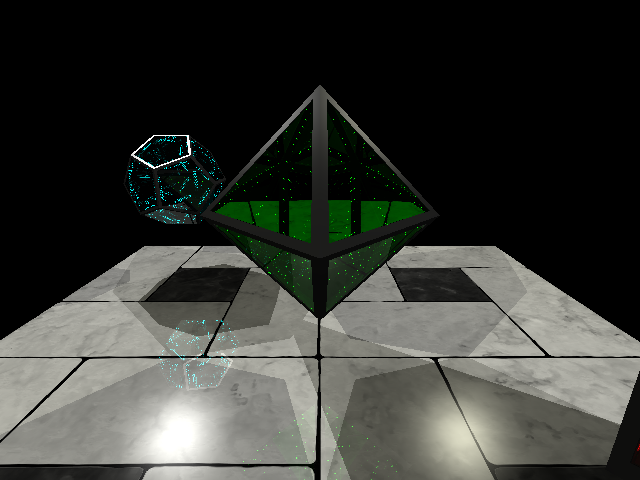
\includegraphics[width=.75\textwidth]{default}
    \caption{Кадр, отрендеренный на $GPU$ без использования $SSAA$}
\end{figure}

\begin{figure}[h!]
    \ContinuedFloat
    \centering
    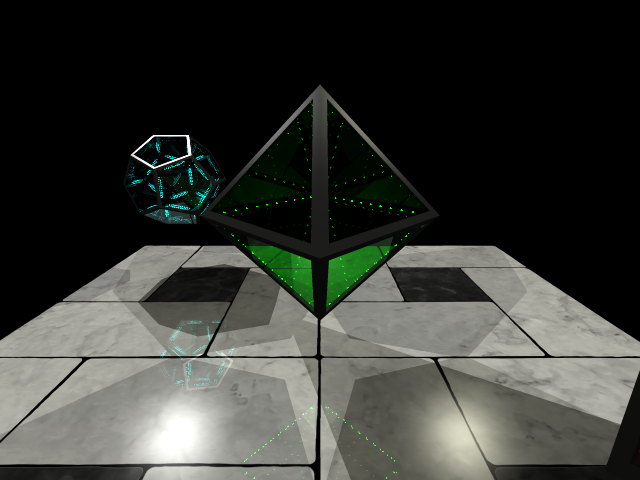
\includegraphics[width=.75\textwidth]{ssaa}
    \caption{Кадр, отрендеренный на $GPU$ с использованием $SSAA$}
\end{figure}

\begin{figure}[h!]
    \ContinuedFloat*
    \centering
    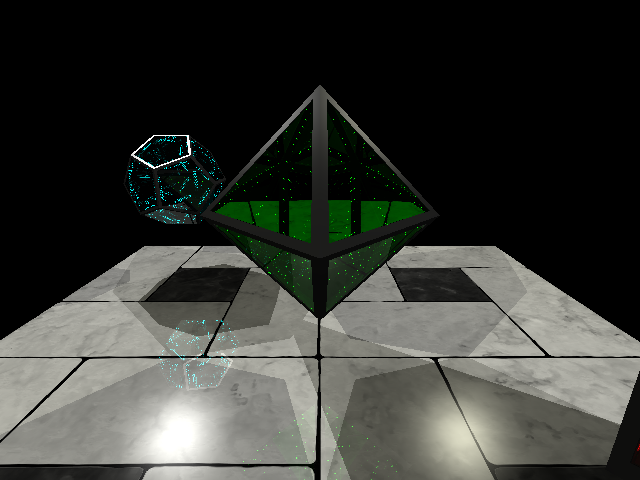
\includegraphics[width=.75\textwidth]{default_cpu}
    \caption{Кадр, отрендеренный на $CPU$ без использования $SSAA$}
\end{figure}

\begin{figure}[h!]
    \ContinuedFloat
    \centering
    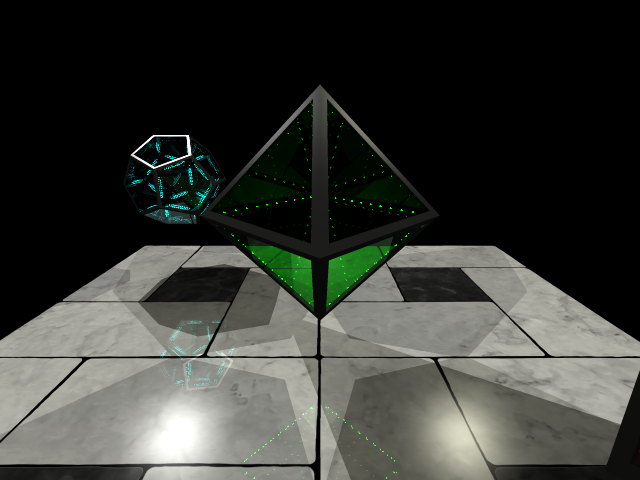
\includegraphics[width=.75\textwidth]{ssaa_cpu}
    \caption{Кадр, отрендеренный на $CPU$ с использованием $SSAA$}
\end{figure}

\end{center}

Невооруженным взглядом можно заметить плавность линий на изображении, построенном с помощью $SSAA$. Также видно, что точность вычислений на $CPU$ и $GPU$ примерно одинаковая, и мы получаем неотличимый результат.

\textbf{Сравнение времени работы}

Неудивительно, что несмотря на многопоточность, используемую в варианте с центральным процессором, вариант с графическим процессором на порядок выигрывает в скорости за счет большего количества потоков.

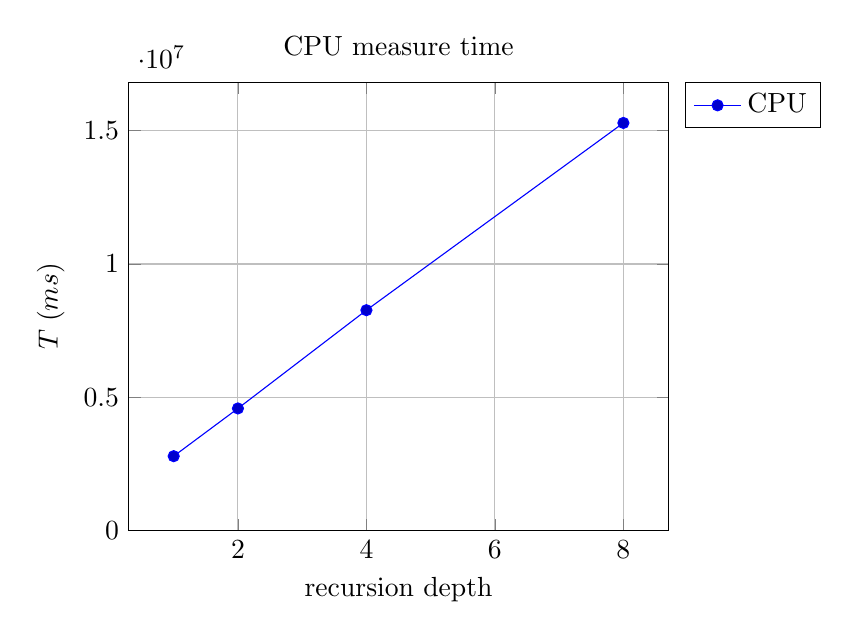
\begin{tikzpicture}% coordinates
	\begin{axis}[
		title = CPU measure time,
		xlabel= recursion depth,
		ylabel= $T\;(ms)$,
		ymin = 0,
		grid=major,
		legend pos = outer north east
		]
		\legend{CPU}
		\addplot coordinates {(1, 2788919) (2, 4580255) (4, 8266978) (8, 15293571)};
	\end{axis}
\end{tikzpicture}

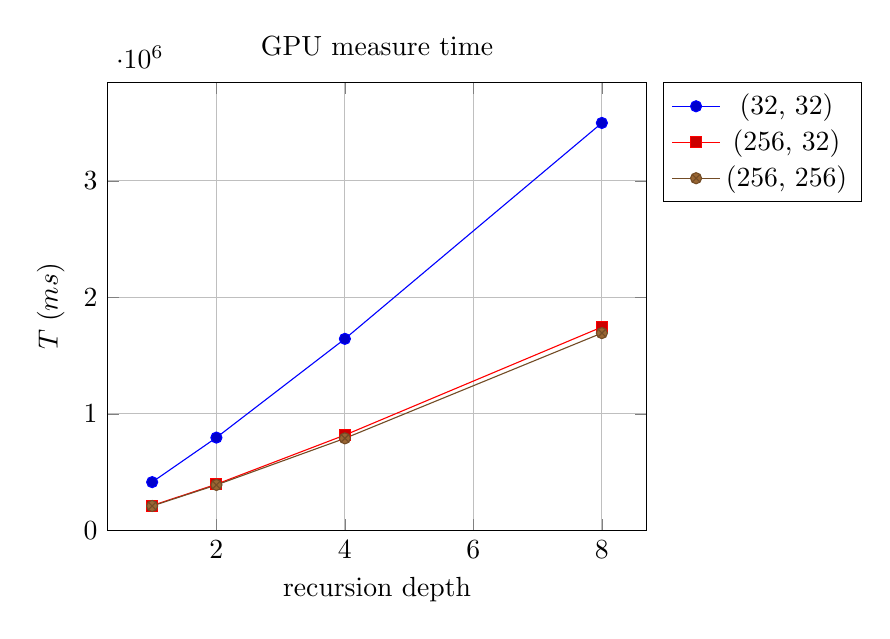
\begin{tikzpicture}% coordinates
	\begin{axis}[
		title = GPU measure time,
		xlabel= recursion depth,
		ylabel= $T\; (ms)$,
		ymin = 0,
		grid=major,
		legend pos = outer north east
		]
		\legend{(32, 32), (256, 32), (256, 256)}
		\addplot coordinates {(1, 415182 ) (2,  797055 ) (4,  1644077) (8, 3496258)};
		\addplot coordinates {(1, 213678 ) (2,  397268 ) (4, 818838) (8,  1745377)};
		\addplot coordinates {(1, 210404 ) (2,  390930 ) (4, 790606) (8, 1693551)};
	\end{axis}
\end{tikzpicture}

\pagebreak